\documentclass[../../../../main.tex]{subfiles}
\begin{document}
\section*{京都大学 1979年 前期}

\begin{flushright}
60/120分
\end{flushright}

\subsection*{第1問}
[解] (i) $p_1(x) = x + a$とおける. (i)に代入して
\[
  \int_{-1}^1 C(x+a) dx = 0 \quad \therefore a = 0
\]
より $p_1(x) = x$

(ii) $p_2(x) = x^2 + ax + b, \ f(x) = \alpha x + \beta$とおく.
\begin{align*}
  &\int_{-1}^1 (x^2+ax+b)(\alpha x+\beta) dx \\
  &= 2\alpha \int_0^1 ax^2 dx + 2\beta \int_0^1 (x^2+b) dx \\
  &= \frac{2}{3}a\alpha + 2\left(\frac{1}{3}+b\right)\beta = 0
\end{align*}
が任意の$\alpha, \beta$で成立するので, $a=0, b=-\frac{1}{3}$となり
\[
  p_2(x) = x^2 - \frac{1}{3}
\]

(iii) $p_3(x) = x^3 + ax^2 + bx + c, \ f(x) = \alpha x^2 + \beta x + \gamma$とおく.
\begin{align*}
  &\int_{-1}^1 p_3(x) f(x) dx \\
  &= 2\alpha \int_0^1 (ax^4+cx^2) dx + 2\beta \int_0^1 (x^4+bx^2) dx + 2\gamma \int_0^1 (ax^2+c) dx \\
  &= 2\left(\frac{1}{5}a+\frac{1}{3}c\right)\alpha + 2\left(\frac{1}{5}+\frac{1}{3}b\right)\beta + 2\left(\frac{1}{3}a+c\right)\gamma \\
  &= 0
\end{align*}
これが全ての$\alpha, \beta, \gamma$で成立するので,
\[
  \begin{cases}
    \frac{1}{5}a + \frac{1}{3}c = 0 \\
    \frac{1}{5} + \frac{1}{3}b = 0 \\
    \frac{1}{3}a + c = 0
  \end{cases}
  \iff
  \begin{cases}
    a=c=0 \\
    b=-\frac{3}{5}
  \end{cases}
\]
だから
\[
  p_3(x) = x^3 - \frac{3}{5}x
\]

\subsection*{第2問}
[解] $x=0, \pi, \pi/2$での成立が必要。又、$0 \le C < 2\pi$とする.
\begin{align}
  3a + b(1+2\cos C - 3\sin C) &= 1 \label{eq2_1} \\
  -a + b(1-2\cos C + 3\sin C) &= 1 \label{eq2_2} \\
  4a + b(1+2\sin C + 3\cos C) &= 1 \label{eq2_3}
\end{align}
以下$\sin C = \alpha$, $\cos C = \beta$とおく. \eqref{eq2_1}+\eqref{eq2_2}から
\begin{equation}
  a + b = 1 \label{eq2_4}
\end{equation}
\eqref{eq2_4}を\eqref{eq2_1}, \eqref{eq2_3}に代入
\begin{align}
  b(-2 + 2\beta - 3\alpha) + 2 &= 0 \label{eq2_5} \\
  b(-3 + 3\beta + 2\alpha) + 3 &= 0 \label{eq2_6}
\end{align}
\eqref{eq2_5}$\times 3$ - \eqref{eq2_6}$\times 2$から
\[
  b[-6 + 6\beta - 9\alpha + 6 - 6\beta - 4\alpha] = 0
\]
\[
  \alpha b = 0
\]
したがって, $b=0$又は$\alpha=0 \iff C=0, \pi$ ($\because 0 \le C < 2\pi$) である.

$1^\circ \ b=0$の時\\
$af(x)=1$が任意の$x$で成立するような$a$は存在せず, 不適.

$2^\circ \ C=0$の時 (この時$\alpha=0, \beta=1$)\\
\eqref{eq2_5}から$2=0$となり不適

$3^\circ \ C=\pi$の時 ($\alpha=0, \beta=-1$)\\
\eqref{eq2_5}から$b=\frac{1}{2}$, \eqref{eq2_4}から$a=\frac{1}{2}$である. 逆にこの時
\[
  \frac{1}{2}f(x) + \frac{1}{2}f(x-\pi) = 1
\]
は任意の$x$について成立し, 十分

以上を, $C$を一般角に直して
\[
  (a, b, C) = \left(\frac{1}{2}, \frac{1}{2}, \pi + 2n\pi\right) \ (n \in \mathbb{Z})
\]

\subsection*{第3問}
[解]
(i) $t > 0$から, AM-GM
\[
  f(t) \ge 2\sqrt{t \cdot \frac{1}{t}} + \sqrt{2\left(t \cdot \frac{1}{t} + 1\right)} = 2 + \sqrt{3}
\]
(等号成立は$t=1$)
\[
  f(t)g(t) = \left(t+\frac{1}{t}+2\right) - \left(t+\frac{1}{t}+1\right) = 1
\]
\[
  \therefore g(t) = \frac{1}{f(t)} \quad (\because f(t) \ge 2+\sqrt{3})
\]
だから, (i)から, $g(t)$は$f(t) = 2+\sqrt{3}$の時, $\max \frac{2-\sqrt{3}}{1}$をとる. 終

(ii) $x, y > 0$から\\
「$a, b, c$を$3$辺とする三角形が常に存在」\\
$\iff$ 「$\frac{a}{\sqrt{xy}}, \frac{b}{\sqrt{xy}}, \frac{c}{\sqrt{xy}} \quad \text{〃}$」\\
である. ここで, $\frac{a}{\sqrt{xy}} = A$などとおき, $t = \frac{x}{y} \ (t>0)$とおくと
\[
  A = \sqrt{t+\frac{1}{t}+1}, \ B = p, \ C = \sqrt{t} + \frac{1}{\sqrt{t}}
\]
まず, (i)から
\begin{equation}
  \max(C-A) = 2-\sqrt{3}, \ \min(A+C) = 2+\sqrt{3} \label{eq3_1}
\end{equation}
だから, もとめる条件は\eqref{eq3_1}が成立するような$A, C$の時での成立が必要で,
\[
  2-\sqrt{3} < p < 2+\sqrt{3}
\]
逆にこの時, $A+C \ge 2+\sqrt{3}, \ C-A \le 2-\sqrt{3}$だから$0 < C-A < p < A+C$となり, たしかに$A, B, C$を3辺とする三角形をつくることが出来, ($\because$ 三角不等式) 十分である.

以上から
\[
  2-\sqrt{3} < p < 2+\sqrt{3}
\]

\subsection*{第4問}
[解]\\
(i)
\[
  p = \sum_{k=1}^6 p_k^2
\]

(ii)
\begin{align}
  p &= p_1^2 + p_2^2 + p_3^2 + p_4^2 + p_5^2 + p_6^2 \label{eq4_1} \\
  1 &= p_1 + p_2 + p_3 + p_4 + p_5 + p_6 \label{eq4_2}
\end{align}

コーシー・シュワルツの不等式から
\[
  (p_1+p_2+p_3+p_4+p_5+p_6)^2 \le 6p
\]
\[
  \therefore p \ge \frac{1}{6} \ (\because \text{\eqref{eq4_2}}) \quad \text{終}
\]
等号成立は$p_1 = p_2 = p_3 = p_4 = p_5 = p_6$の時で, \eqref{eq4_2}からこの時
\[
  p_k = \frac{1}{6}
\]
である 終

\subsection*{第5問}
[解] 点$X$に対し, $\overrightarrow{OX} = \vec{x}$と定めると, $|\vec{a}_k| = \text{const} \ (k=1 \sim 6)$

\begin{center}
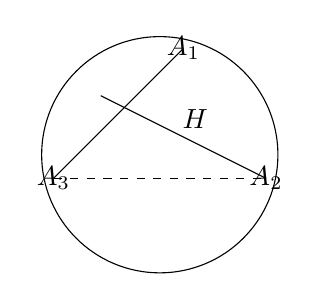
\begin{tikzpicture}[scale=1.5]
  \draw (0,0) circle (1);
  \node at (0.2, 0.9) {$A_1$};
  \node at (0.9, -0.2) {$A_2$};
  \node at (-0.9, -0.2) {$A_3$};
  \draw (0.2, 0.9) -- (-0.9, -0.2);
  \draw (0.9, -0.2) -- (-0.5, 0.5);
  \node at (0.3, 0.3) {$H$};
  \draw[dashed] (-0.9, -0.2) -- (0.9, -0.2);
\end{tikzpicture}
\end{center}

(i)
\begin{align*}
  &\overrightarrow{A_2H} \cdot \overrightarrow{A_1A_3} \\
  &= (\vec{a}_1+\vec{a}_3) \cdot (\vec{a}_3-\vec{a}_1) \\
  &= |\vec{a}_3|^2 - |\vec{a}_1|^2 = 0
\end{align*}
より $A_2H \perp A_1A_3$

同様にして, 各頂点と$H$を通る直線と, その対辺が直交するから$H$は垂心である 終

(ii) 選んだ3点$A_a, A_b, A_c$, のこりの3点$A_D, A_E, A_F$とする
(集合$\{A, B, \cdots, F\} = \{1, 2, 3, \cdots, 6\}$). (i)から$\triangle A_aA_bA_c$の垂心$H$は
\begin{equation}
  \vec{h} = \vec{a}_a + \vec{a}_b + \vec{a}_c \label{eq5_1}
\end{equation}
又, $\triangle A_DA_EA_F$の重心$G$として
\begin{equation}
  \vec{g} = \frac{1}{3} (\vec{a}_D + \vec{a}_E + \vec{a}_F) \label{eq5_2}
\end{equation}
\eqref{eq5_1}, \eqref{eq5_2}から$G, H$を通る直線上の点$X$は, $t \in \mathbb{R}$として
\[
  \vec{x} = \frac{1}{3} (\vec{a}_D + \vec{a}_E + \vec{a}_F) + \frac{t}{3} (3\vec{a}_a + 3\vec{a}_b + 3\vec{a}_c - \vec{a}_D - \vec{a}_E - \vec{a}_F)
\]
と表せる. $t = \frac{1}{4}$として
\[
  \vec{x} = \frac{1}{4} (\vec{a}_a + \cdots + \vec{a}_F) = \frac{1}{4} \sum_{k=1}^6 \vec{a}_k
\]
これは3点のえらび方によらないから, 題意は示された 終

\subsection*{第6問}
(行列)
\end{document}
